\documentclass{article}
\usepackage{graphicx} 

\title{ID2090 ASSIGNMENT-4}
\author{Madhan M \\CH22B078}
\date{14-June 2023}

\begin{document}

\maketitle

\section{Introduction}
The Fourier series is a mathematical tool that allows us to represent a periodic function as an infinite sum of sine and cosine functions. It was introduced by the French mathematician Jean-Baptiste Joseph Fourier in the early 19th century and has since become a fundamental concept in mathematics, physics, and engineering.Many natural phenomena and signals in various fields, such as sound, light, and electrical waveforms, exhibit periodic behavior. In this document, we will explore the concept of Fourier series and its mathematical formulation.
\section{WHAT IS A FOURIER SERIES?}
 A Fourier series is an expansion of a periodic function f(x) in terms of an infinite sum of sines and cosines. It is used to decompose any periodic function into the sum of a set of simple oscillating functions, namely sines and cosines. Fourier Series makes use of the orthogonality relationships of the sine and cosine functions.\\
  \textbf{In short,A Fourier Series is a Approximation for a Periodic Function.} 
  \\
  \\
  A general equation of Fourier series is represented by the following equation:\\
  \\
\[
f(t) = a_0 + \sum_{n=1}^{\infty} \left(a_n \cos\left(\frac{2\pi n t}{T}\right) + b_n \sin\left(\frac{2\pi n t}{T}\right)\right)
\]

where \(a_0\), \(a_n\), and \(b_n\) are the Fourier coefficients. The coefficients can be calculated using the following formulas:

\[
a_0 = \frac{1}{T} \int_{-T/2}^{T/2} f(t) \, dt
\]

\[
a_n = \frac{2}{T} \int_{-T/2}^{T/2} f(t) \cos\left(\frac{2\pi n t}{T}\right) \, dt
\]
\\
\[
b_n = \frac{2}{T} \int_{-T/2}^{T/2} f(t) \sin\left(\frac{2\pi n t}{T}\right) \, dt
\]

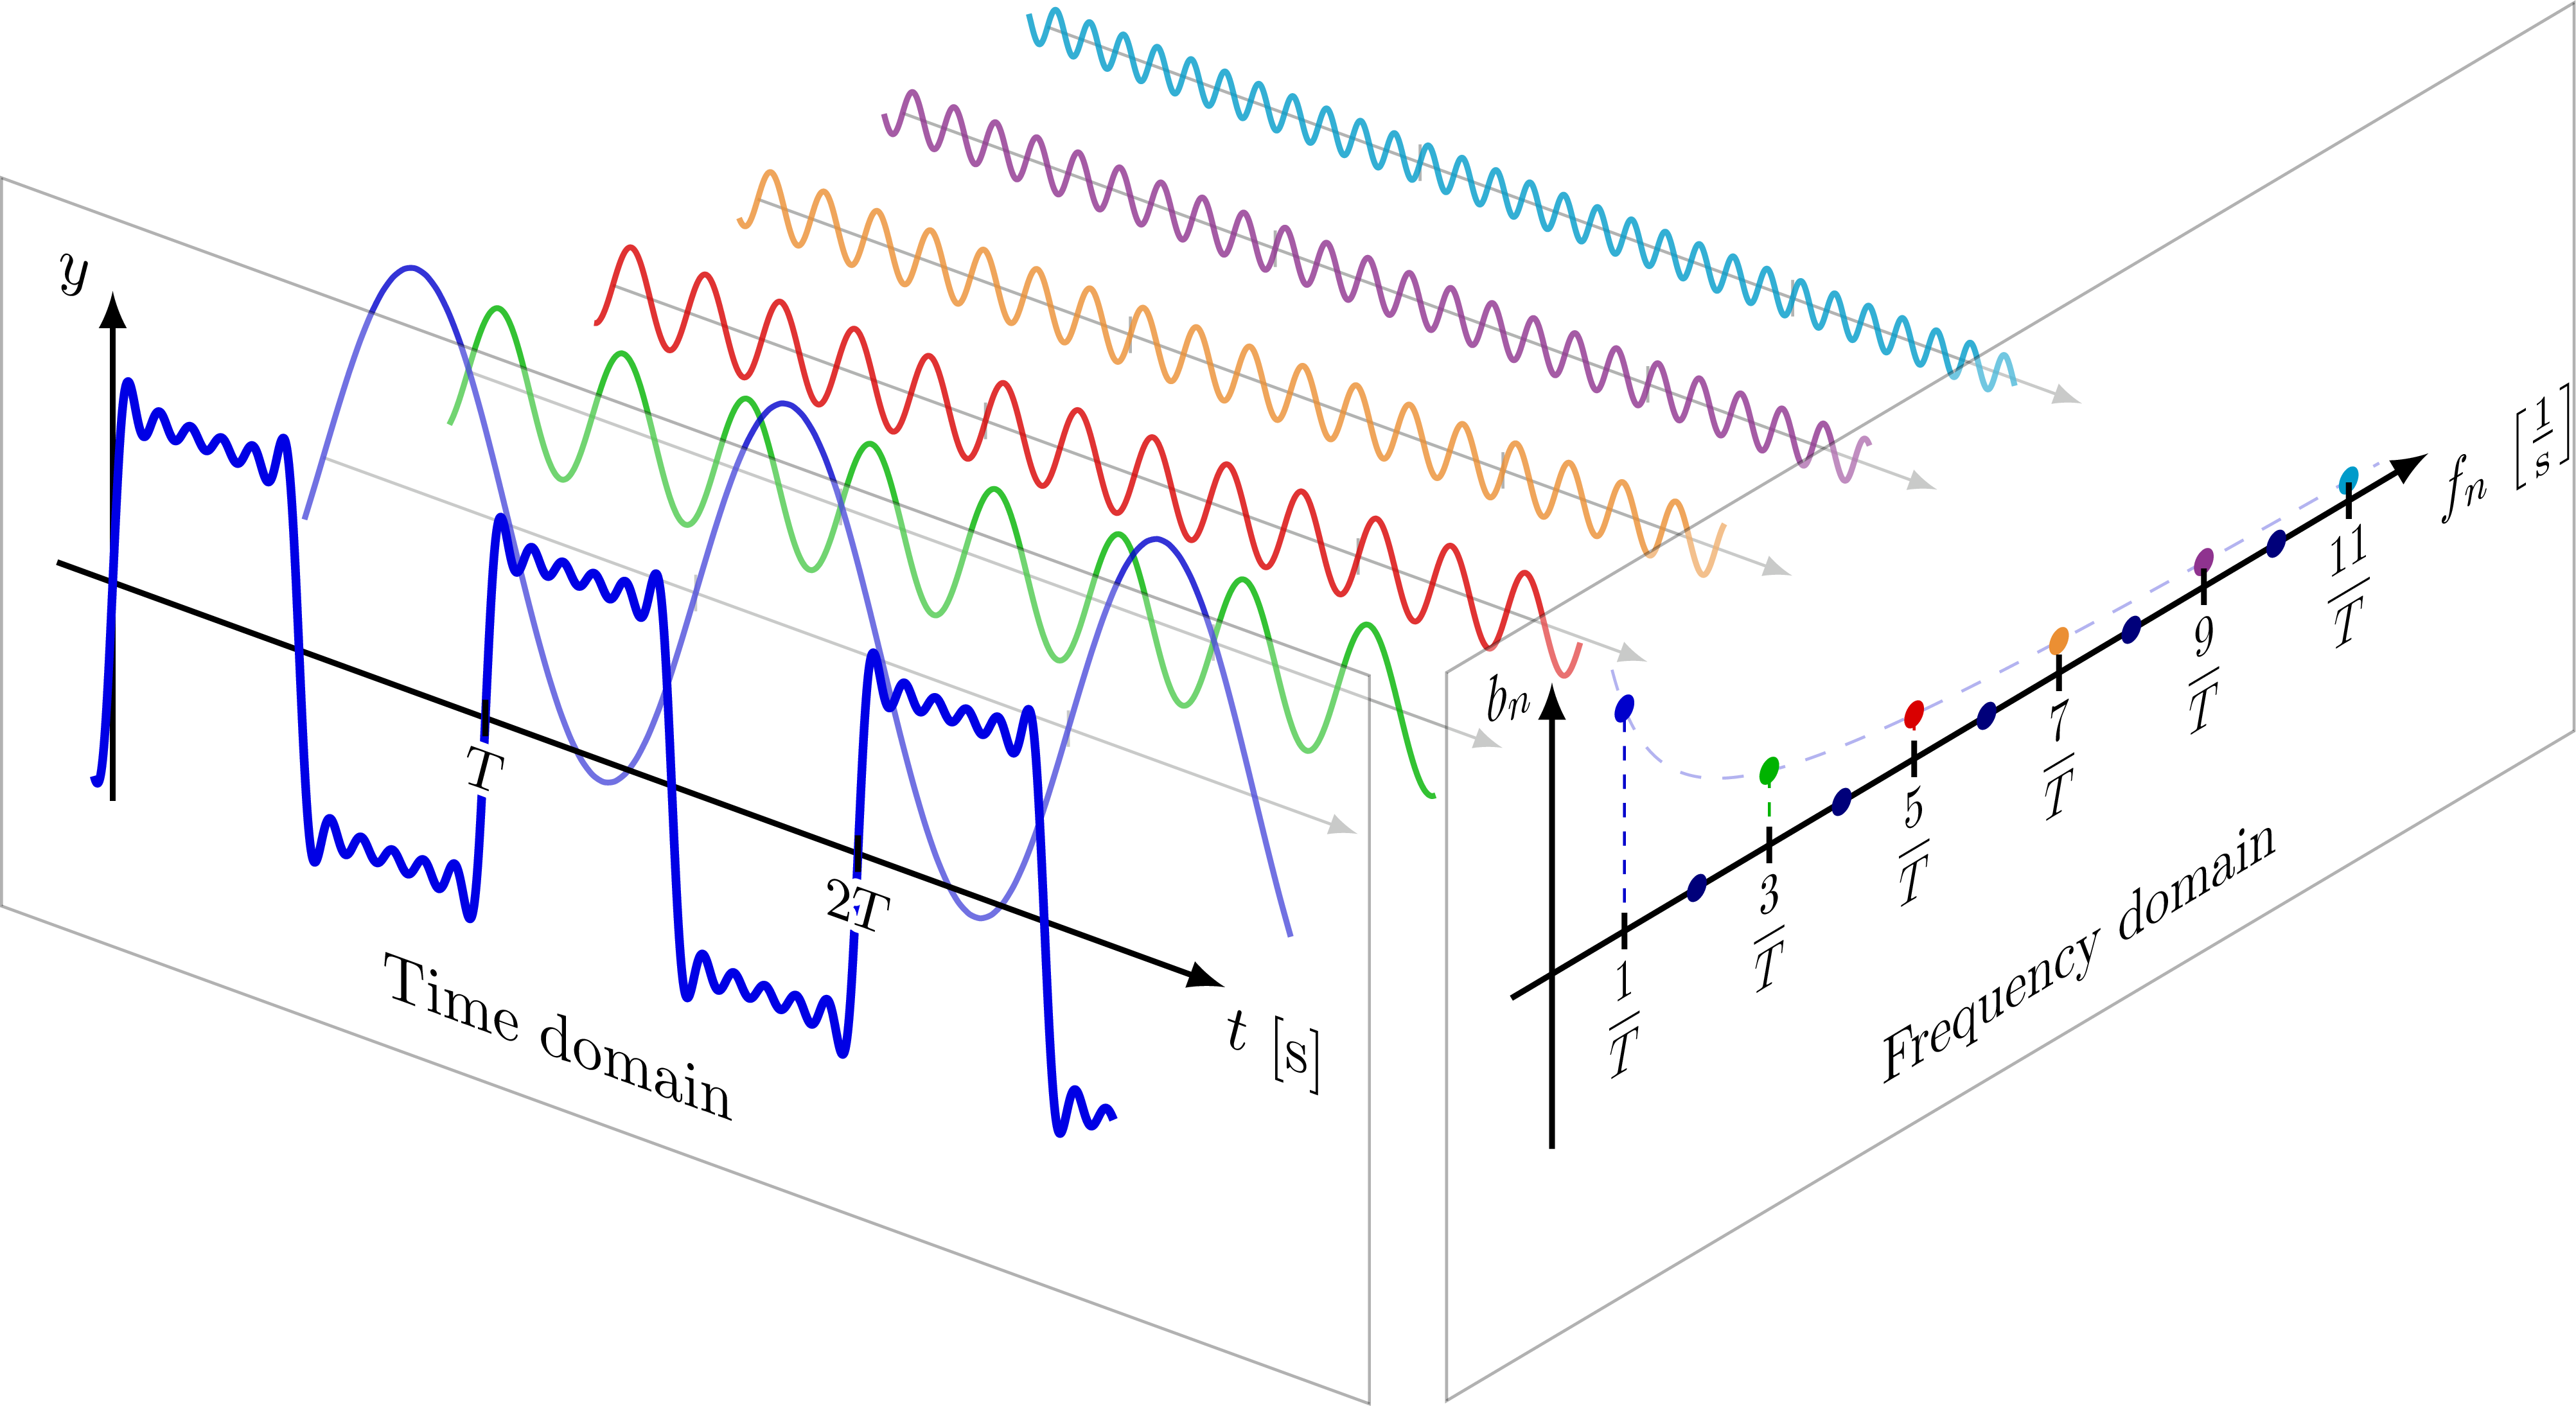
\includegraphics[width=0.8\textwidth]{Fourier2.png}
\\
\section{PROPERTIES OF FOURIER SERIES}
Some Important properties of Fourier series:
\begin{itemize}
\item Fourier series is primarily used to periodic functions
\item Fourier series is a linear operation, which means that the sum of two periodic functions.
\item The sine and cosine functions used in Fourier series are orthogonal over a period. 
\item  Fourier series may converge or diverge depending on the  function .Functions generally converge to the original function (in case of discontinuities,Function converges at midpoint). 
\item If a function is even (symmetric about the y-axis) or odd (asymmetric about the y-axis), the Fourier series coefficients are simplified in the Integral. For even functions, only cosine terms appear in the series, while for odd functions, only sine terms appear.\\
For even Functions:\\
\[ a_0 = \frac{2}{T} \int_{0}^{\frac{T}{2}} f(t) \, dt \]

\[ a_n = \frac{4}{T} \int_{0}^{\frac{T}{2}} f(t) \cos\left(\frac{2\pi n t}{T}\right) \, dt \]
\[ b_n = 0 \]\\
For Odd Function:\\
\[ a_0 = 0 \]
\[ a_n = 0 \]
\[ b_n = \frac{4}{T} \int_{0}^{\frac{T}{2}} f(t) \sin\left(\frac{2\pi n t}{T}\right) \, dt \]

 \item When a Fourier series approximates a function with a jump discontinuity or sharp corner, oscillations known as the Gibbs phenomenon can occur. These oscillations are a characteristic feature of Fourier series approximations.
 \end{itemize}

\section{APPLICATION OF FOURIER SERIES:}
The Fourier series has a wide range of applications in various fields for approximating Function.These Include:\\
 Fourier Series plays an Important role in Electrical and Communication systems:

\begin{itemize}
\item Circuit Analysis:It is employed in circuit analysis to understand the behavior of periodic electrical waveforms. By representing periodic signals using Fourier series, complex waveforms can be decomposed into their constituent frequencies. 
\item Signal Analysis: It is extensively used in signal processing for analyzing and manipulating signals. It allows signals to be represented in the frequency domain, where various operations like filtering, compression, modulation, and demodulation can be performed more efficiently.
\item Image Analysis:It plays a crucial role in image processing and computer vision. It is used for tasks such as image enhancement, image compression, edge detection, and image reconstruction.

\end{itemize}
\footnote{I have looked up this from "Fourier Series Transformation" in MA1102
 Course}
 
\end{document}
